% secciones/analitico_agéntico.tex

\section{Análisis Agéntico}

\subsection{Arquitectura del sistema}

La capa agéntica implementada sigue el paradigma de \textit{skills}, donde cada componente
encapsula una responsabilidad específica del pipeline. El sistema recibe una pregunta en
lenguaje natural y produce una tabla de resultados ejecutando SQL sobre el Data Warehouse
retail en Spark.

El pipeline completo se compone de cuatro skills ejecutados en secuencia:

\begin{enumerate}[noitemsep]
    \item \textbf{Clasificador de intención} — identifica el tipo de análisis solicitado
          mediante coincidencia de palabras clave en la pregunta.
    \item \textbf{Generador SQL} — invoca la API de Gemini con el esquema de las cinco
          tablas y la pregunta del usuario, obteniendo una consulta SQL compatible con Spark SQL.
    \item \textbf{Ejecutor de consulta} — ejecuta el SQL generado sobre el Data Warehouse
          retail mediante una \texttt{SparkSession} con soporte Hive.
    \item \textbf{Formateador de resultado} — serializa el DataFrame resultante a JSON
          con tipos de datos normalizados para su consumo por el frontend.
\end{enumerate}

\begin{figure}[H]
    \centering
    \includegraphics[width=0.85\textwidth]{figuras/pipeline_agéntico.png}
    \caption{Pipeline del sistema agéntico: de lenguaje natural a resultado sobre Spark.}
\end{figure}

\subsection{Generación de SQL con Gemini}

El skill de generación SQL utiliza el modelo \texttt{gemini-1.5-flash} de Google.
El prompt de sistema incluye el esquema completo de las cinco tablas y restricciones
sobre el formato de salida:

\begin{lstlisting}[style=python, caption={Configuración del prompt para generación de SQL}]
PROMPT_SISTEMA = f"""
Eres un experto en SQL y analisis de datos retail.
Tu unica tarea es generar consultas SQL compatibles con Spark SQL
a partir de preguntas en lenguaje natural.

{ESQUEMA}

Reglas:
- Responde UNICAMENTE con la consulta SQL, sin explicaciones.
- No uses bloques de codigo markdown, solo el SQL puro.
- Usa alias descriptivos en espanol para las columnas.
- Incluye USE retail; al inicio de cada consulta.
"""
\end{lstlisting}

\subsection{Dashboard web}

El dashboard fue implementado con FastAPI como backend y HTML/CSS/JS como frontend.
La interfaz permite ingresar preguntas en lenguaje natural y visualizar el pipeline
de procesamiento en tiempo real.

\begin{figure}[H]
    \centering
    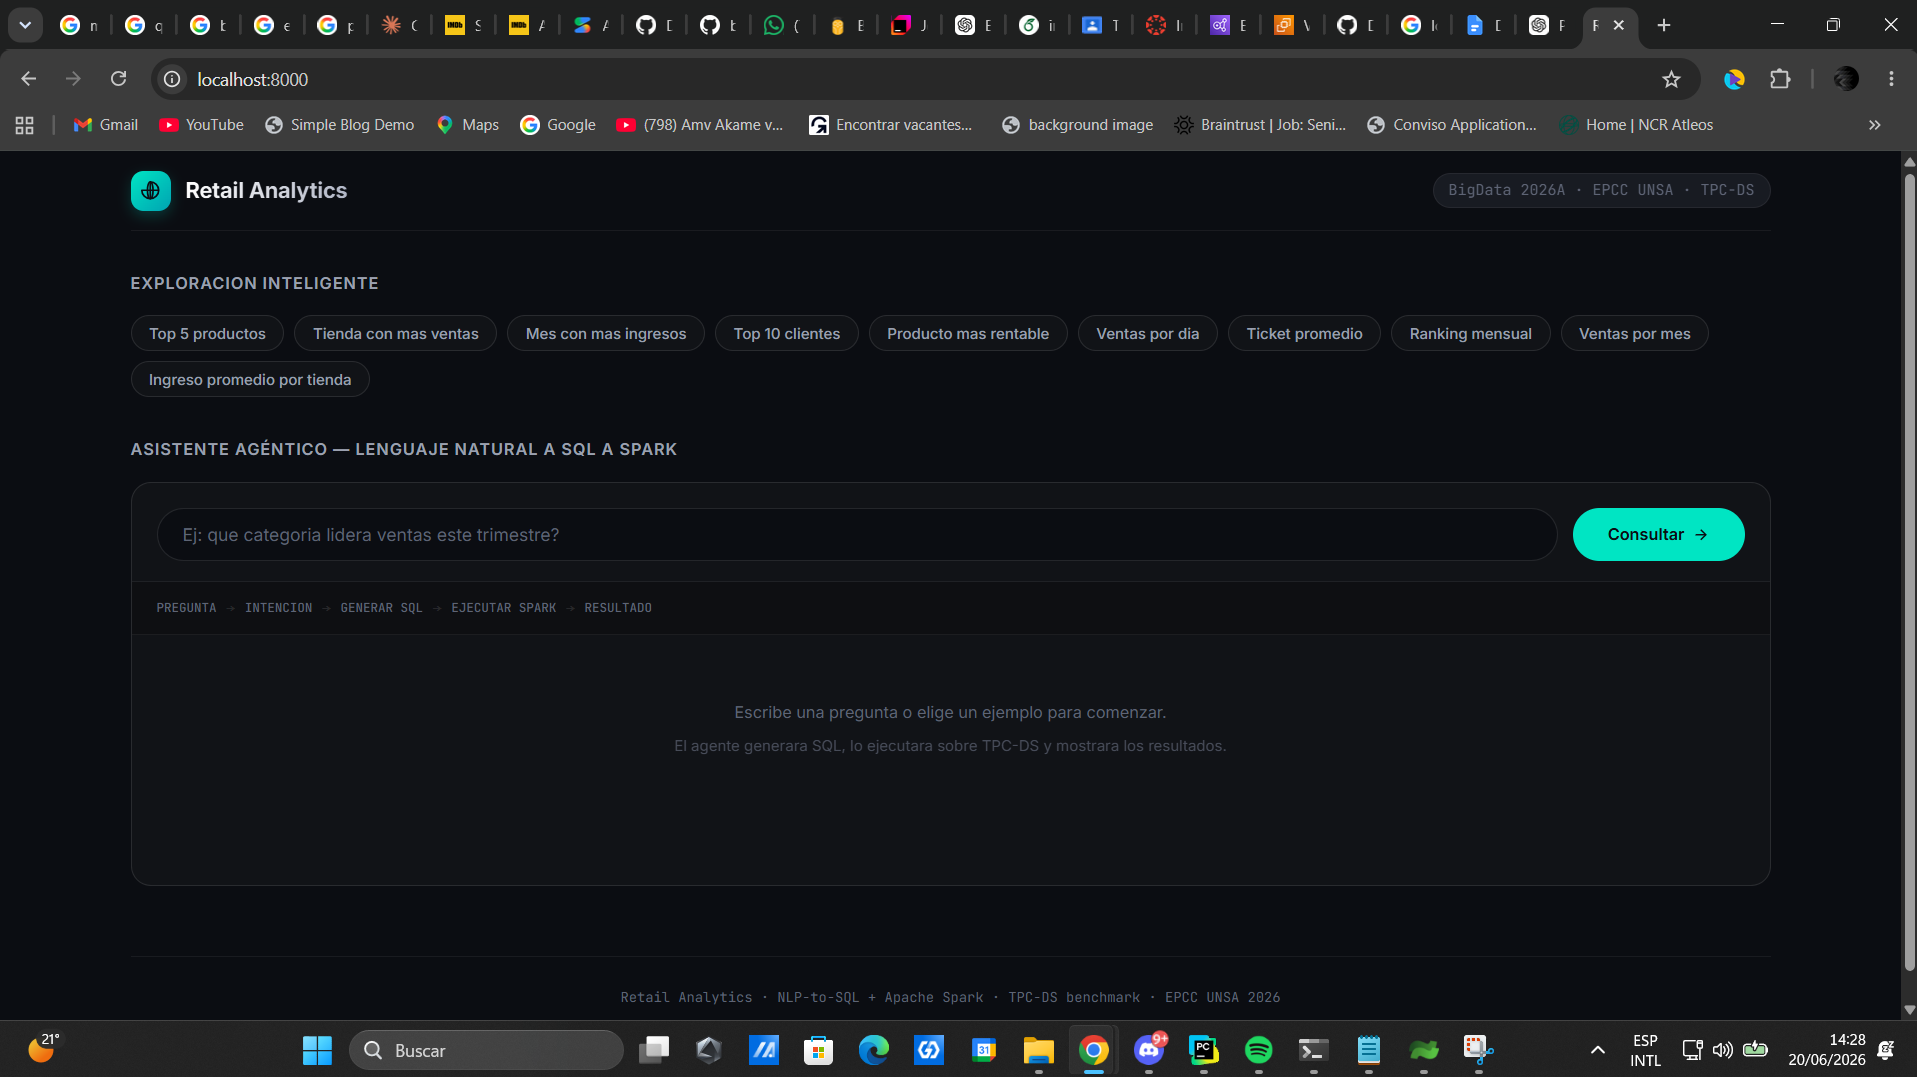
\includegraphics[width=0.92\textwidth]{figuras/dashboard_principal.png}
    \caption{Dashboard principal: chips de consultas rápidas y área de chat agéntico.}
\end{figure}

\begin{figure}[H]
    \centering
    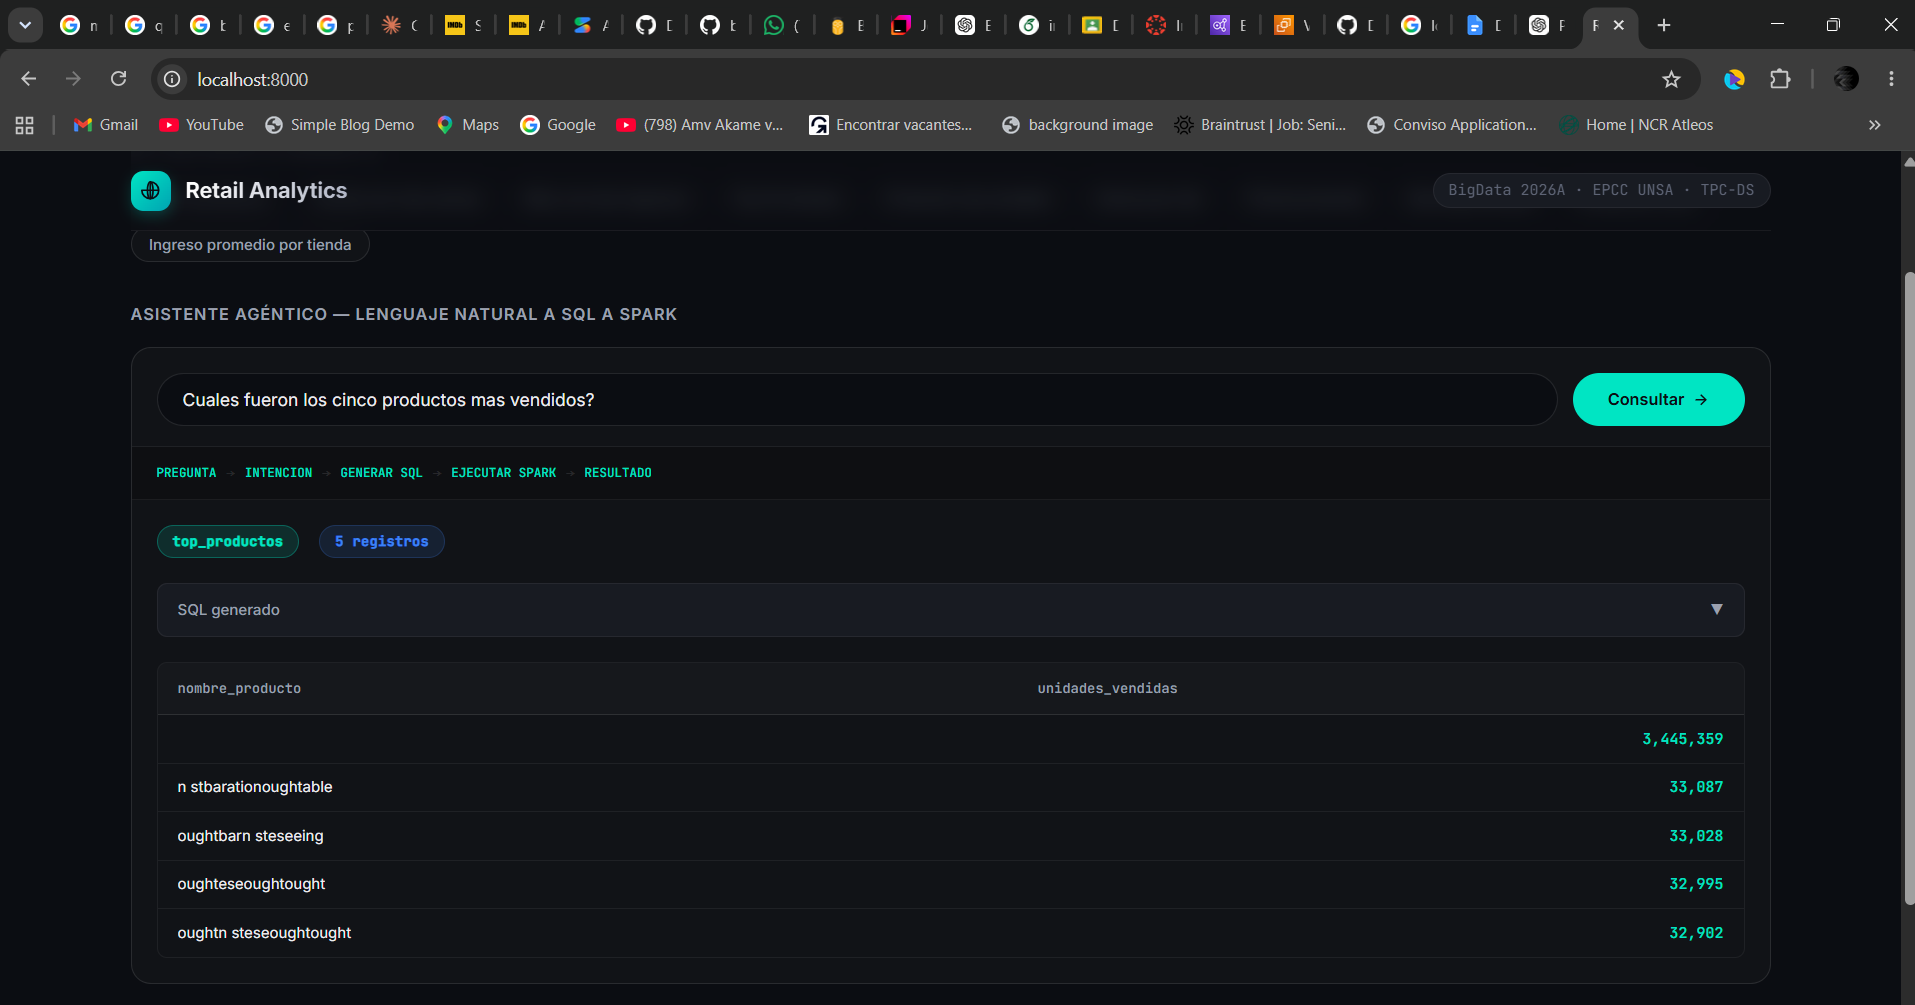
\includegraphics[width=0.92\textwidth]{figuras/dashboard_resultado.png}
    \caption{Resultado de una consulta agéntica: badge de intención, SQL generado expandible y tabla de resultados.}
\end{figure}

\subsection{Consultas agénticas ejecutadas}

\begin{table}[H]
    \centering
    \caption{Consultas en lenguaje natural y SQL generado por Gemini}
    \label{tab:agéntico}
    \begin{tabularx}{\textwidth}{l X}
        \toprule
        \textbf{Pregunta en lenguaje natural} & \textbf{Intención identificada} \\
        \midrule
        ¿Cuáles fueron los cinco productos más vendidos?   & top\_productos \\
        ¿Qué tienda tuvo mayores ventas?                   & ventas\_tienda \\
        ¿Cuál fue el mes con mayores ingresos?             & ventas\_mes \\
        ¿Cuáles son los diez mejores clientes?             & top\_clientes \\
        ¿Qué producto generó mayores ingresos?             & productos\_ingresos \\
        ¿Cuáles son las ventas por día de la semana?       & ventas\_dia \\
        ¿Cuál es el ticket promedio por cliente?           & ticket\_promedio \\
        ¿Cuál es el ranking mensual de tiendas?            & ranking\_mensual \\
        ¿Cuáles son las ventas totales por mes?            & ventas\_mes \\
        ¿Qué tienda tiene mayor ingreso promedio?          & ventas\_tienda \\
        \bottomrule
    \end{tabularx}
\end{table}

\subsection{Comparación: consulta manual vs análisis agéntico}

\begin{table}[H]
    \centering
    \caption{Comparación entre consulta manual y análisis agéntico}
    \label{tab:manual_vs_agéntico}
    \begin{tabularx}{\textwidth}{l X X}
        \toprule
        \textbf{Aspecto} & \textbf{Consulta manual} & \textbf{Análisis agéntico} \\
        \midrule
        Conocimiento requerido  & SQL, HiveQL o PySpark    & Lenguaje natural \\
        Tiempo de formulación   & Minutos                  & Segundos \\
        Flexibilidad            & Total (cualquier query)  & Limitada al esquema TPC-DS \\
        Riesgo de error SQL     & Depende del analista     & Depende del modelo LLM \\
        Trazabilidad            & El analista conoce el SQL & SQL visible en la interfaz \\
        Escalabilidad           & Un analista por sesión   & Múltiples usuarios simultáneos \\
        \bottomrule
    \end{tabularx}
\end{table}

\subsection{Limitaciones del enfoque agéntico}

El sistema agéntico implementado presenta las siguientes limitaciones:

\begin{itemize}[noitemsep]
    \item El clasificador de intención basado en palabras clave no cubre preguntas
          con formulaciones muy distintas a las previstas.
    \item Gemini puede generar SQL sintácticamente válido pero semánticamente incorrecto
          si la pregunta es ambigua o hace referencia a columnas inexistentes.
    \item El tiempo de respuesta del agente incluye la latencia de la API de Gemini
          y el tiempo de ejecución en Spark, lo que puede ser mayor que una consulta
          manual precompilada.
    \item El sistema no mantiene contexto entre preguntas, por lo que cada consulta
          se procesa de forma independiente.
\end{itemize}
